%
% File acl2017.tex
%
%% Based on the style files for ACL-2015, with some improvements
%%  taken from the NAACL-2016 style
%% Based on the style files for ACL-2014, which were, in turn,
%% based on ACL-2013, ACL-2012, ACL-2011, ACL-2010, ACL-IJCNLP-2009,
%% EACL-2009, IJCNLP-2008...
%% Based on the style files for EACL 2006 by 
%%e.agirre@ehu.es or Sergi.Balari@uab.es
%% and that of ACL 08 by Joakim Nivre and Noah Smith

\documentclass[11pt,a4paper]{article}
\usepackage[hyperref]{acl2017}
\usepackage{times}
\usepackage{latexsym}
\usepackage[pdftex]{graphicx}

\usepackage{url}

%\aclfinalcopy % Uncomment this line for the final submission
%\def\aclpaperid{***} %  Enter the acl Paper ID here

%\setlength\titlebox{5cm}
% You can expand the titlebox if you need extra space
% to show all the authors. Please do not make the titlebox
% smaller than 5cm (the original size); we will check this
% in the camera-ready version and ask you to change it back.

\newcommand\BibTeX{B{\sc ib}\TeX}

\title{Midterm project report for the Natural Language Understanding Systems course}

\author{Federico Giuggioloni \\
  189662 \\
  {\tt federico.giuggioloni@studenti.unitn.it}}

\date{}

\begin{document}
\maketitle
\begin{abstract}
  This work provides a concept tagging tool for queries related to movies, such as "who is the director of thor".
  The final version of the script enables tweaking of various learning parameters to better evaluate which setting is the best for the situation.
  % TODO Write which version achieves the best F1 score
\end{abstract}

\section{Introduction}

\section{Data set analysis}

% Dataset explanation, similar to README
The dataset is subdivided into a training set and a test set.
These sets are in a word per line format, with the sentences being separated by an empty line.
Multiple columns represent the features of the specific word (such as part-of-speech tag and the lemma) and the correct concept tag.

An analysis of the distribution of the data provided was deemed necessary to ensure it's correct usage.

\subsection{Zipf's law}

The first analysis performed on the training data is to check whether or not Zipf's law is verified.
Due to the nature of the data, a bias towards words typical of the movie industry was expected.
This can be seen clearly in the word frequency distribution, with "movies" and "movie" occupying respectively the second and fifth spot.
(with "movies" appearing more frequently than "of")

%Histogram that shows Zipf's law in action
\begin{figure}[h]
\centering
  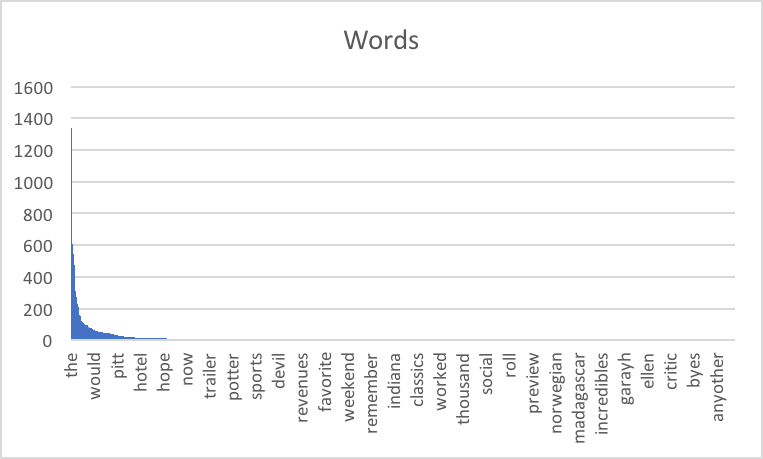
\includegraphics[width=.9\linewidth]{Images/zipf}
  \caption{Zipf's law}
\label{fig:zipf}
\end{figure}


\subsection{Concept distribution}

The most frequent concept is "movie.name" by a wide margin, which means this plus out-of-span tags make up 86\% of the tags present in the training dataset.

%Histogram with concept distribution and generalization distribution
\begin{figure}[h]
\centering
  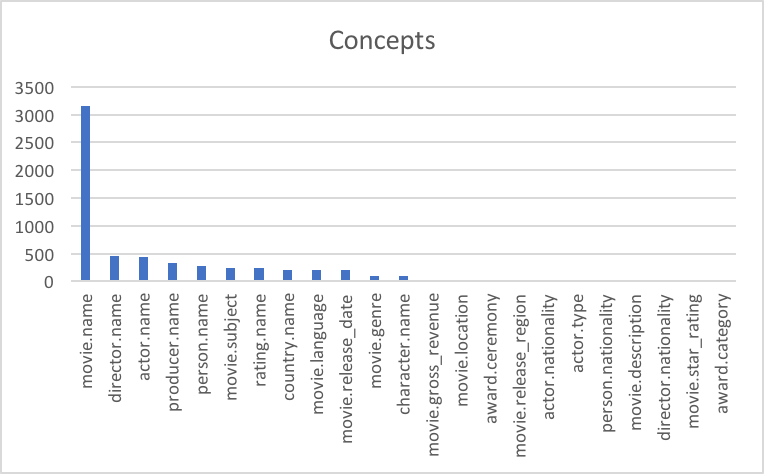
\includegraphics[width=.9\linewidth]{Images/concepts}
  \caption{Concept distribution}
\label{fig:zipf}
\end{figure}

\section{Baseline solution}
The case of a single transducer from word to concept will be taken in consideration as the baseline for all the proposed solutions.
This doesn't take into consideration the structure of the phrase so it is expected to be very inaccurate. 

\begin{verbatim}
accuracy:  67.32%
precision:  20.15%
recall:  54.72%
FB1:  29.45
\end{verbatim}

The resulting F1-Score is very low as expected.

\section{Direct solution}

The simplest and most direct method is obtained by simply composing the transducer from the previous step with the concept model trained on the training data.
To do this the training data was converted from word-per-row to a concept sentence-per-row format. These sentences have been used to train a wide array of language models, by changing the order of the n-grams and the smoothing method.

It can be observed that using a language model trained on bigrams achieves better performance than one trained on trigrams, which can be explained by looking at the training and test sets.
% TODO need to check this A few concept tags only appear as bigrams in the training corpus, while they appear only as trigrams in the test one.

\subsection{Witten bell, 3-grams}
\begin{verbatim}
accuracy:  92.62%
precision:  76.58%
recall:  74.61%
FB1:  75.58
\end{verbatim}

\subsection{Witten bell, 2-grams}
\begin{verbatim}
Smoothing method: witten_bell
Order: 2-grams
accuracy:  92.68%
precision:  78.51%
recall:  74.34%
FB1:  76.37
\end{verbatim}

\section{Solution using extra features}

The next experiment was to try and include the extra features included in the dataset to improve the F1-Score.
At a first glance the chaining of multiple transducers, each passing from one feature to the next, seemed like a good idea.
Because of this 3 transducers were built and composed: word-to-lemma, lemma-to-part of speech, part of speech-to-concept tag.
By composing the result with the concept model it is shown to be even worse than the baseline:

\begin{verbatim}
Smoothing method: witten_bell
Order: 2-grams
accuracy:  72.81%
precision:  27.35%
recall:   6.14%
FB1:  10.03
\end{verbatim}

An explanation can be found by considering that this method is reducing the input space of the final transducer from the size of the vocabulary to just 38 pos-tags.

Because of this, a second method which keeps the first transducer, while replacing the second and third with a lemma-to-concept transducer.
The second transducer takes into consideration the pos-tags in the calculation of the weights.

\begin{verbatim}
Smoothing method: witten_bell
Order: 3-grams
accuracy:  92.34%
precision:  76.06%
recall:  73.97%
FB1:  75.00
\end{verbatim}

The performance of this method is comparable to the version without extra features.


\section{Solution with generalization}
As the inclusion of the extra features does not seem to improve performance this method does not use them.

The idea was to create two transducers, one that transforms words into a generalization (a word class), while the second transduces from a word class to a concept. The method was implemented by pre-processing the training set, adding a "word class" column created as a derivative of the concept tag. Because of this, including the fact that the only acceptable generalization does nothing more than remove the IOB part of the tags, the performance is lower than the standard method:
\begin{verbatim}
Smoothing method: witten_bell
Order: 3-grams
accuracy:  88.70%
precision:  61.42%
recall:  61.14%
FB1:  61.28
\end{verbatim}

\section{Using frequency cut-off}

%Thoughts and F1-Score

\section{Conclusion}



\subsection{Sections}

If you are using the provided \LaTeX{} and Bib\TeX{} style files, you
can use the command \verb|\citet| (cite in text)
to get ``author (year)'' citations.

If the Bib\TeX{} file contains DOI fields, the paper
title in the references section will appear as a hyperlink
to the DOI, using the hyperref \LaTeX{} package.
To disable the hyperref package, load the style file
with the \verb|nohyperref| option:
\verb|\usepackage[nohyperref]{acl2017}|

As examples, we cite \cite{P16-1001} to show you how papers with a DOI
will appear in the bibliography.  We cite \cite{C14-1001} to show how
papers without a DOI but with an ACL Anthology Identifier will appear
in the bibliography.  

As reviewing will be double-blind, the submitted version of the papers
should not include the authors' names and affiliations. Furthermore,
self-references that reveal the author's identity, {\em e.g.},
\begin{quote}
``We previously showed \cite{Gusfield:97} ...''  
\end{quote}
should be avoided. Instead, use citations such as 
\begin{quote}
``\citeauthor{Gusfield:97} \shortcite{Gusfield:97}
previously showed ... ''
\end{quote}

\textbf{Please do not use anonymous citations} and do not include
acknowledgements when submitting your papers. Papers that do not
conform to these requirements may be rejected without review.

\textbf{References}: Gather the full set of references together under
the heading {\bf References}; place the section before any Appendices,
unless they contain references. Arrange the references alphabetically
by first author, rather than by order of occurrence in the text.
Provide as complete a citation as possible, using a consistent format,
such as the one for {\em Computational Linguistics\/} or the one in the 
{\em Publication Manual of the American 
Psychological Association\/}~\cite{APA:83}.  Use of full names for
authors rather than initials is preferred.  A list of abbreviations
for common computer science journals can be found in the ACM 
{\em Computing Reviews\/}~\cite{ACM:83}.

The \LaTeX{} and Bib\TeX{} style files provided roughly fit the
American Psychological Association format, allowing regular citations, 
short citations and multiple citations as described above.

{\bf Appendices}: Appendices, if any, directly follow the text and the
references (but see above).  Letter them in sequence and provide an
informative title: {\bf Appendix A. Title of Appendix}.



% include your own bib file like this:
%\bibliographystyle{acl}
%\bibliography{acl2017}
\bibliography{acl2017}
\bibliographystyle{acl_natbib}

\appendix

\section{Supplemental Material}
\label{sec:supplemental}
ACL 2017 also encourages the submission of supplementary material
to report preprocessing decisions, model parameters, and other details
necessary for the replication of the experiments reported in the 
paper. Seemingly small preprocessing decisions can sometimes make
a large difference in performance, so it is crucial to record such
decisions to precisely characterize state-of-the-art methods.

Nonetheless, supplementary material should be supplementary (rather
than central) to the paper. {\bf Submissions that misuse the supplementary 
material may be rejected without review.}
Essentially, supplementary material may include explanations or details
of proofs or derivations that do not fit into the paper, lists of
features or feature templates, sample inputs and outputs for a system,
pseudo-code or source code, and data. (Source code and data should
be separate uploads, rather than part of the paper).

The paper should not rely on the supplementary material: while the paper
may refer to and cite the supplementary material and the supplementary material will be available to the
reviewers, they will not be asked to review the
supplementary material.

Appendices ({\em i.e.} supplementary material in the form of proofs, tables,
or pseudo-code) should come after the references, as shown here. Use
\verb|\appendix| before any appendix section to switch the section
numbering over to letters.

\section{Multiple Appendices}
\dots can be gotten by using more than one section. We hope you won't
need that.

\end{document}
